\documentclass[journal]{IEEEtran}
\usepackage[a5paper, margin=10mm]{geometry}
%\usepackage{lmodern} % Ensure lmodern is loaded for pdflatex
\usepackage{tfrupee} % Include tfrupee package


\setlength{\headheight}{1cm} % Set the height of the header box
\setlength{\headsep}{0mm}     % Set the distance between the header box and the top of the text


%\usepackage[a5paper, top=10mm, bottom=10mm, left=10mm, right=10mm]{geometry}

%
\usepackage{gvv-book}
\usepackage{gvv}
\setlength{\intextsep}{10pt} % Space between text and floats

\makeindex

\begin{document}
\bibliographystyle{IEEEtran}
\onecolumn
\newpage
\title{Assignment-  9-9.3-7}
\author{AI24BTECH11004-Bheri Sai Likith Reddy}
\maketitle
\textbf{Question}:
Find the area of the region enclosed by the curves $y^2=x, x=\frac{1}{4},y=0 $ and $x=1.$
\hfill{(12,2022)}\\
\solution
The general equation of a parabola with directrix $\vec{n}^{\top}\vec{x}=c$ is given by,
\begin{align}
	g\brak{\vec{x}}=\vec{x}^{\top}\vec{V}\vec{x}+2\vec{u}^{\top}\vec{x}+f=0\\
	\vec{V}=\norm{\vec{n}}^2\vec{I}-e^2\vec{n}\vec{n}^{\top}\\
	\vec{u}=ce^2\vec{n}-\norm{\vec{n}}^2\vec{F}\\
	f=\norm{\vec{n}}^2\norm{\vec{F}}^2-c^2e^2
\end{align}
for the parabola $y^2=x$, equation of the directrix is $\myvec{-1&0}\vec{x}=\frac{1}{4}$
\begin{align}
	\vec{V}&=\myvec{0&0\\0&1}\\
	\vec{u}&=\myvec{\frac{-1}{2}\\0}\\
	f&=0
\end{align}
for the line x-$\frac{1}{4}=0$, parameters are 
\begin{align}
	h_2=\myvec{\frac{1}{4}\\ 0}\\
	m=\myvec{0\\1}
\end{align}
we know that the points of intersection of the line 
\begin{align}
      \vec L: \vec x= \vec h +\kappa \vec m\\
\end{align}	
with the conic section $g\brak{\vec{x}}=\vec{x}^{\top}\vec{V}\vec{x}+2\vec{u}^{\top}\vec{x}+f=0$ is given by $\vec x_i=\vec h +\kappa_i \vec m$
where $$\kappa _i=\frac{1}{\vec m ^T\vec V \vec m}\brak{-\vec m^T\brak{\vec V \vec h + \vec U} +- \sqrt{\sbrak{\vec m ^T\brak{\vec V \vec h +\vec u}}^2-g\brak{h}\brak{\vec m^T \vec V \vec m}}}$$
from this we get $k_i=1,-1$\\
That implies that the points of intersections are $a_0=\myvec{\frac{1}{4}\\ \frac{1}{2}}$ and $a_1=\myvec{\frac{1}{4}\\ \frac{-1}{2}}$\\
similarly for line $x=1$ we get point of intersections as $a_3=\myvec{1\\1}$ and $a_2=\myvec{1\\-1}$\\
hence area of the region between the two lines and the parabola and the x axis is  
$$\int_\frac{1}{4}^1\sqrt{x}dx-\int^1_\frac{1}{4} 0dx=\frac{7}{12}$$
\begin{table}[h!]
	\centering
	\begin{tabular}{|c|p{5cm}|}
\hline
Point & Description \\  \hline
$a_0(0.25,0.5),a_0(0.25,0.5)$ &Point of intersection of the line x=0.25 and the parabola $y^2=x$ \\
	\hline
$a_2(1,1),a_3(1,-1)$ &Point of intersection of the line x=0.25 and the parabola $y^2=x$ Point of intersection of the line x=1 and the parabola $y^2=x$  \\  
	\hline
\end{tabular}


\end{table}
\begin{figure}[h!]
    \centering
    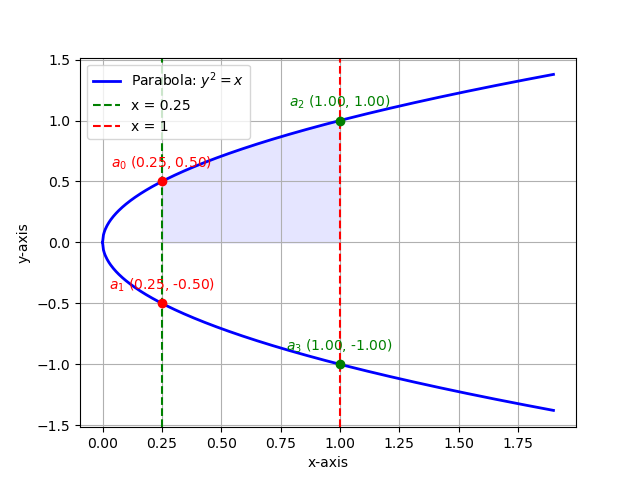
\includegraphics[width=0.7\textwidth]{figs/figasgn3.png}
\end{figure}

\end{document}
